\subsection{点分布}

在本节中，X 表示一个 \(C^{r}\) 类流形，x 是 X 的一个点。

13.2.1. 设 \(\mathcal{A}\) 为由对 \((c, t)\) 组成的集合，其中 \(c = (\mathrm{U}, \varphi, \mathrm{E})\) 是 X 的以 \(x\) 为中心的卡，且 \(t \in \mathrm{TS}^{(r)}(\mathrm{E})\)。称 \(((\mathrm{U}, \varphi, \mathrm{E}), t)\) 与 \(((\mathrm{U}', \varphi', \mathrm{E}'), t')\) 这两个 \(\mathcal{A}\) 的元素等价，如果 \(t' = \gamma_*(t)\)，其中 \(\gamma = \varphi' \circ \varphi^{-1}\)。这样就得到 \(\mathcal{A}\) 上的一个等价关系；该关系的一个等价类称为 X 上点 \(x\) 处的点分布。

设 \(\mathrm{T}_{x}^{(r)}(\mathrm{X})\) 为 X 上点 x 处的点分布全体组成的集合。若 c 是 X 的以 x 为中心的一个卡，则映射

\[
\theta_ {c} \colon \mathsf {T S} ^ {(r)} (\mathrm{E}) \to \mathbf {T} _ {x} ^ {(r)} (\mathrm{X})
\]

把 \(t\) 映为 \((c, t)\) 的类，它是一个双射。在后续内容中，我们给 \(\mathrm{T}_{x}^{(r)}(\mathrm{X})\) 装备把 \(\mathrm{TS}^{(r)}(\mathrm{E})\) 的结构经由 \(\theta_{c}\) 转移而得到的 K-向量空间结构；该结构与 \(c\) 的选取无关。类似地，若 \(k \leqslant r\)，我们用 \(\mathrm{T}_{x}^{(k)}(\mathrm{X})\) 和 \(\mathrm{T}_{x}^{(k)+}(\mathrm{X})\) 表示 \(\mathrm{TS}^{(k)}(\mathrm{E})\) 与 \(\mathrm{TS}^{(k)+}(\mathrm{E})\) 在 \(\theta_{c}\) 下的像；它们与 \(c\) 的选取无关。\(\mathrm{T}_{x}^{(r)}(\mathrm{X})\) 的元素称为阶 \(\leqslant k\) 的，如果它属于 \(\mathrm{T}_{x}^{(k)}(\mathrm{X})\)。我们有

\[
\mathbf {T} _ {x} ^ {(k)} (\mathbf {X}) = \mathbf {T} _ {x} ^ {(0)} (\mathbf {X}) \oplus \mathbf {T} _ {x} ^ {(k) +} (\mathbf {X}).
\]

存在唯一的一个元素 \(\varepsilon_x\) 属于 \(\mathrm{T}_x^{(0)}(\mathbf{X})\)，使得 \(\theta_c(1) = \varepsilon_x\) 对卡 \(c\)（\(\mathbf{X}\) 的以 \(x\) 为中心的卡）成立。若 \(t\) 是点 \(x\) 处的一个点分布，我们称 \(t\) 的常数项为元素 \(\lambda\)（属于 \(\mathbf{K}\)），使得 \(t - \lambda \varepsilon_x \in \mathrm{T}_x^{(r)+}(\mathbf{X})\)；若其常数项为零，则称 \(t\) 不含常数项。

13.2.2. 设 F 是一个分离的多项式空间，f 是定义在 x 的一个邻域上、取值于 F 的 \(C^{r}\) 类函数。设 t 是 X 上点 x 处的一个点分布。

取 X 的一个卡 \(c = (\mathrm{U}, \varphi, \mathrm{E})\)，其中心为 \(x\)，并令 \(f_c = f \circ \varphi^{-1}\)，\(t_c = \theta_c^{-1}(t)\)；由 13.1.3 定义的 F 中元素 \(\langle f_c, t_c \rangle\) 与 \(c\) 的选取无关；我们把它记作 \(\langle f, t \rangle\)。我们有 \(\varepsilon_x(f) = f(x)\)。\(^{(1)}\) \(t\) 的常数项是 \(\langle 1, t \rangle\)。

若 \(\mathbf{F}'\) 是一个分离的多范数空间，且 \(u: \mathbf{F} \to \mathbf{F}'\) 连续且线性，则我们有 \(\langle u \circ f, t \rangle = u(\langle f, t \rangle)\)。

假设 F 是一个 Banach 空间，且 t 的阶 \(\leqslant k\)，其中 k 有限。设 \(j \in \mathrm{J}_{x}^{k}(\mathrm{X}, \mathrm{F})\)（参见 12.1.2），并设 \(f \in j\)。那么 \(\langle f, t \rangle\) 只依赖于射流 j；我们把它记作 \(\langle j, t \rangle\)。这样定义的从 \(\mathrm{T}_{x}^{(k)}(\mathrm{X}) \times \mathrm{J}_{x}^{k}(\mathrm{X}, \mathrm{F})\) 到 F 的映射是双线性的。当 F = K 时，我们已令 \(\mathrm{J}_{x}^{k}(\mathrm{X}, \mathrm{F}) = \mathrm{P}_{x}^{k}(\mathrm{X})\)（参见 12.6.2），从而得到 \(\mathrm{T}_{x}^{(k)}(\mathrm{X}) \times \mathrm{P}_{x}^{k}(\mathrm{X})\) 上的一个双线性形式。

13.2.3. 设 \(\varphi: X \to Y\) 是一个 \(C^r\) 类流形态射，且 \(y = \varphi(x)\)。设 \(c = (U, \psi, E)\) 是 \(X\) 的以 \(x\) 为中心的卡，\(c' = (U', \psi', E')\) 是 \(Y\) 的以 \(y\) 为中心的卡；设 \(\bar{\varphi}\) 是 \(\varphi\) 在这些卡中的表达式（5.3.2），并设 \(\bar{\varphi}_*\) 是从 \(\mathrm{TS}^{(r)}(E)\) 到 \(\mathrm{TS}^{(r)}(E')\) 的相应映射（参见 13.1.4）。存在唯一的线性映射，记作 \(\mathrm{T}_x^{(r)}(\varphi)\) 或 \(\varphi_*\)，它把 \(\mathrm{T}_x^{(r)}(X)\) 映到 \(\mathrm{T}_y^{(r)}(Y)\)，且使该图交换

\pandocbounded{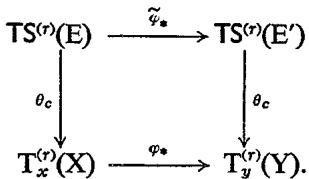
\includegraphics[keepaspectratio]{images/part001_e22e7577.jpg}}

该映射与 \(c\) 和 \(c'\) 的选取无关。若 \(t \in \mathrm{T}_{x}^{(r)}(\mathbf{X})\)，则称 \(\varphi_{*}(t)\) 为 \(t\) 经 \(\varphi\) 得到的像。我们有 \(\varphi_{*}(\varepsilon_{x}) = \varepsilon_{y}\)。若 \(k \leqslant r\)，则有

\[
\varphi_ {*} (\mathrm{T} _ {x} ^ {(k)} (\mathrm{X})) \subset \mathrm{T} _ {y} ^ {(k)} (\mathrm{Y}) \quad \text { and } \quad \varphi_ {*} (\mathrm{T} _ {x} ^ {(k) +} (\mathrm{X})) \subset \mathrm{T} _ {y} ^ {(k) +} (\mathrm{Y}).
\]

若 \(\varphi': X \to Y\) 是一个 \(C^r\) 类态射，且满足 \(\varphi'(x)=y\)，则 \(\varphi_* = \varphi_*'\) 当且仅当 \(j_x^r(\varphi) = j_x^r(\varphi')\)（参见 12.1）。

若 \(\varphi\) 在 \(x, \varphi_*\) 处是一个浸入（相应地，一个浸没），则它是单射（相应地，满射）；当 \(\dim_y Y < +\infty\) 时逆命题成立。

若 \(\varphi'\colon\mathbf{Y}\to\mathbf{Z}\) 是一个 \(\mathbf{C}^{r}\) 类流形态射，且 \(t\in\mathbf{T}_{x}^{(r)}(\mathbf{X})\)，则有 \((\varphi'\circ\varphi)_{*}(t)=\varphi_{*}^{\prime}(\varphi_{*}(t))\)。

设 F 是一个分离的多范数空间，f 是定义在 y 的一个邻域上、取值于 F 的 \(C^{r}\) 类函数。此时我们有

\[
\langle f, \varphi_ {*} (t) \rangle = \langle f \circ \varphi , t \rangle \quad \text {   for   all   } \quad t \in \mathrm{T} _ {x} ^ {(r)} (\mathrm{X}).\tag{1}
\]

对给定的 \(t\)，关系式 (1)（其中 \(f\) 与 \(F\) 为变量）刻画了 \(\varphi_{*}(t)\)；当 \(\dim_y Y < +\infty\) 时，可以只限于 \(F = K\) 的情形。

13.2.4. 假设 X 是 Banach 空间 E 的一个开子流形。用 \(\varphi_x\) 表示从 X 到 E 的映射 \(y \mapsto y - x\)；卡 \(c = (X, \varphi_x, E)\) 以 \(x\) 为中心。于是 \(\mathrm{T}_x^{(r)}(\mathbf{X})\) 与 \(\mathrm{TS}^{(r)}(\mathbf{E})\) 通过 \(\theta_c^{-1}\) 恒同。特别地，我们有 \(\mathrm{T}_x^{(\infty)}(\mathbf{X}) = \mathrm{TS}(\mathbf{E})\)。

设 F 是一个 Banach 空间，\(u: E \to F\) 是一个连续线性映射，且 \(x \in E\)，\(y \in F\) 满足 \(u(x) = y\)。如上所述，把 \(\mathrm{T}_{x}^{(\infty)}(E)\) 与 TS(E) 恒同，把 \(\mathrm{T}_{y}^{(\infty)}(F)\) 与 TS(F) 恒同。映射

\[
u _ {*} \colon \mathrm{TS(E)} \rightarrow \mathrm{TS(F)} \quad (\text { cf. } 13.2.3)
\]

与由 u 到张量代数的典范扩张所诱导的映射 TS(u) 一致。

13.2.5. 若 \(k \leqslant r\)，用 \(\mathrm{T}^{(k)}(\mathrm{X})\)（相应地，\(\mathrm{T}^{(k)+}(\mathrm{X})\)）表示诸 \(\mathrm{T}_a^{(k)}(\mathrm{X})\)（相应地，诸 \(\mathrm{T}_a^{(k)+}(\mathrm{X})\)，其中 \(a \in \mathrm{X}\)）的集合和。映射 \(t: \mathrm{X} \to \mathrm{T}^{(k)}(\mathrm{X})\) 若满足 \(t(a) \in \mathrm{T}_a^{(k)}(\mathrm{X})\)（对一切 \(a \in \mathrm{X}\)），则称为阶 \(\leqslant k\) 的点分布场。

假设 \(k\) 有限且 X 局部有限维。对每个 \(a \in X\)，双线性形式 \((j, t) \mapsto \langle j, t \rangle\)（参见 13.2.2）定义了一个同构 \(i_a\)，它把 \(\mathrm{T}_a^{(k)}(\mathrm{X})\) 映到 \(\mathrm{P}_a^k(\mathrm{X})^*\) 即 \(\mathrm{P}_a^k(\mathrm{X})\) 的对偶上。这些 \(i_a\) 定义了一个双射 \(i: \mathrm{T}^{(k)}(\mathrm{X}) \to \mathrm{P}^k(\mathrm{X})^*\)，其中 \(\mathrm{P}^k(\mathrm{X})^*\) 表示向量丛 \(\mathrm{P}^k(\mathrm{X})\) 的对偶；经由 \(i^{-1}\) 转移结构，我们给 \(\mathrm{T}^{(k)}(\mathrm{X})\) 装备一个以 X 为底、类为 \(\mathbf{C}^{r-k}\) 的向量丛结构。阶 \(\leqslant k\) 的点分布场称为 \(\mathbf{C}^s\) 类的（其中 \(s \leqslant r - k\)），如果它是 \(\mathbf{C}^s\) 类截面，即丛 \(\mathrm{T}^{(k)}(\mathrm{X})\) 的截面。

设 \(\varphi\colon\mathbf{X}\to\mathbf{Y}\) 是一个 \(\mathbf{C}^{r}\) 类流形态射，并假设 Y 与 X 一样是局部有限维的。那么 \(\varphi_{*}\colon\mathrm{T}^{(k)}(\mathrm{X})\to\mathrm{T}^{(k)}(\mathrm{Y})\) 是一个向量丛的 \(\varphi\)-态射，其类为 \(\mathbf{C}^{r-k}\)。

13.2.6. 设 \(k\) 是满足 \(0 \leqslant k \leqslant r\) 的整数。若 U 是有限维 Banach 空间 E 的一个开集，则依据 13.2.4，向量丛 \(\mathbf{T}^{(k)}(\mathbf{U})\) 与以 \(\mathbf{TS}^{(k)}(\mathbf{E})\) 为纤维的平凡丛恒同。

特别地，取 \(E = K^n\)，其中 \(n \geqslant 0\)，并设 \((e_1, \ldots, e_n)\) 为 \(E\) 的典范基。若 \(\alpha = (\alpha_1, \ldots, \alpha_n)\) 是 \(N^n\) 的一个元素，用 \(\Delta^\alpha\) 表示元素 \(\gamma_{\alpha_1}(e_1) \ldots \gamma_{\alpha_n}(e_n)\)（\(TS(E)\) 中的元素，所用的乘积是对称张量的对称积，参见 A, IV, § 5, no. 3）。\(^{(1)}\) 诸 \(\Delta^\alpha\)（其中 \(|\alpha| \leqslant k\)）构成 \(TS^{(k)}(E)\) 的一个基；若 \(a \in K^n\)，用 \(\Delta_a^\alpha\) 表示 \(T_a^{(k)}(E)\) 中相应的元素。设 F 是一个分离的多范数空间，f 是 \(C^r\) 类、定义在 \(a\) 的一个邻域内且取值于 F 的函数；若 \(\alpha \in N^n\)，则元素 \(\langle f, \Delta_a^\alpha \rangle\) 与 2.5.3、3.2.1 和 4.2.1 中定义的元素 \((\Delta^\alpha f)(a)\) 一致。

假设 X 局部有限维，并设 \(\xi = (\xi^1, \ldots, \xi^n)\) 是 X 在开集 U 上的一个坐标系。若 \(a \in \mathbf{U}\) 且 \(\alpha\) 是满足 \(|\alpha| \leqslant k\) 的多重指标，则用 \((\Delta_{\xi}^{\alpha})_a\) 表示点 \(a\) 处这样的点分布：它在 \(\xi\) 下的像是点分布 \(\Delta_{\xi(a)}^{\alpha}\)（在 \(\mathbf{K}^n\) 上）；分布场

\[
\Delta_ {\xi} ^ {\alpha}: a \mapsto (\Delta_ {\xi} ^ {\alpha}) _ {a} \quad (| \alpha | \leqslant k)
\]

构成向量丛 \(\mathbf{T}^{(k)}(\mathbf{X})\) 在 U 上的一个标架。若 \(f\colon \mathbf{U}\to \mathbf{F}\) 是 \(\mathbf{C}^r\) 类的，我们令 \(\langle f, (\Delta_{\xi}^{\alpha})_a\rangle = \Delta_{\xi}^{\alpha}f(a)\)，并用 \(\Delta_{\xi}^{\alpha}f\) 表示函数 \(a\mapsto \Delta_{\xi}^{\alpha}f(a)\)；它是 U 上的一个 \(\mathbf{C}^{r - k}\) 类函数。

\(^{1}\) 若 \(m = |\alpha|\)，且 \(\Sigma\) 是映射 \(\sigma\)（从 \(\{1, \ldots, m\}\) 到 \(\{1, \ldots, n\}\)、满足 \(\operatorname{Card}\sigma^{-1}(i)=\alpha_i\)）全体的集合，则有

\[
\Delta^ {\alpha} = \gamma_{\alpha_1}(e_1) \dots \gamma_{\alpha_n}(e_n) = \sum_{\sigma \in \Sigma} e_{\sigma(1)} \otimes \dots \otimes e_{\sigma(n)}, \quad \text { cf. A, IV, } \S 5, \text { no. } 4.
\]

